CMake项目变大时,配置可能会花费相当长的时间,特别是当加载了外部内容或需要对工具链特性进行大量检查时。优化的第一步是检查配置过程的哪一部分占用了多少时间。从3.18版本开始,CMake包含了命令行选项来生成漂亮的分析图,以调查配置过程中花费的时间。通过使用-{}-profiling-output和-{}-profiling-format分析标志,CMake将创建分析输出。编写本书时,仅支持输出格式的Google跟踪格式,但还是需要指定格式和文件来创建分析信息。调用CMake来创建一个概要图可以这样操作:

\begin{tcblisting}{commandshell={}}
cmake -S <sourceDir> -B <buildDir> --profiling-output
  ./profiling.json --profiling-format=google-trace
\end{tcblisting}

当前目录下,将分析数据输出到profiling.json文件中。通过在地址栏中输入about://tracing,可以使用Google Chrome查看输出文件。本书缓存的GitHub项目的输出如下所示:

\begin{center}
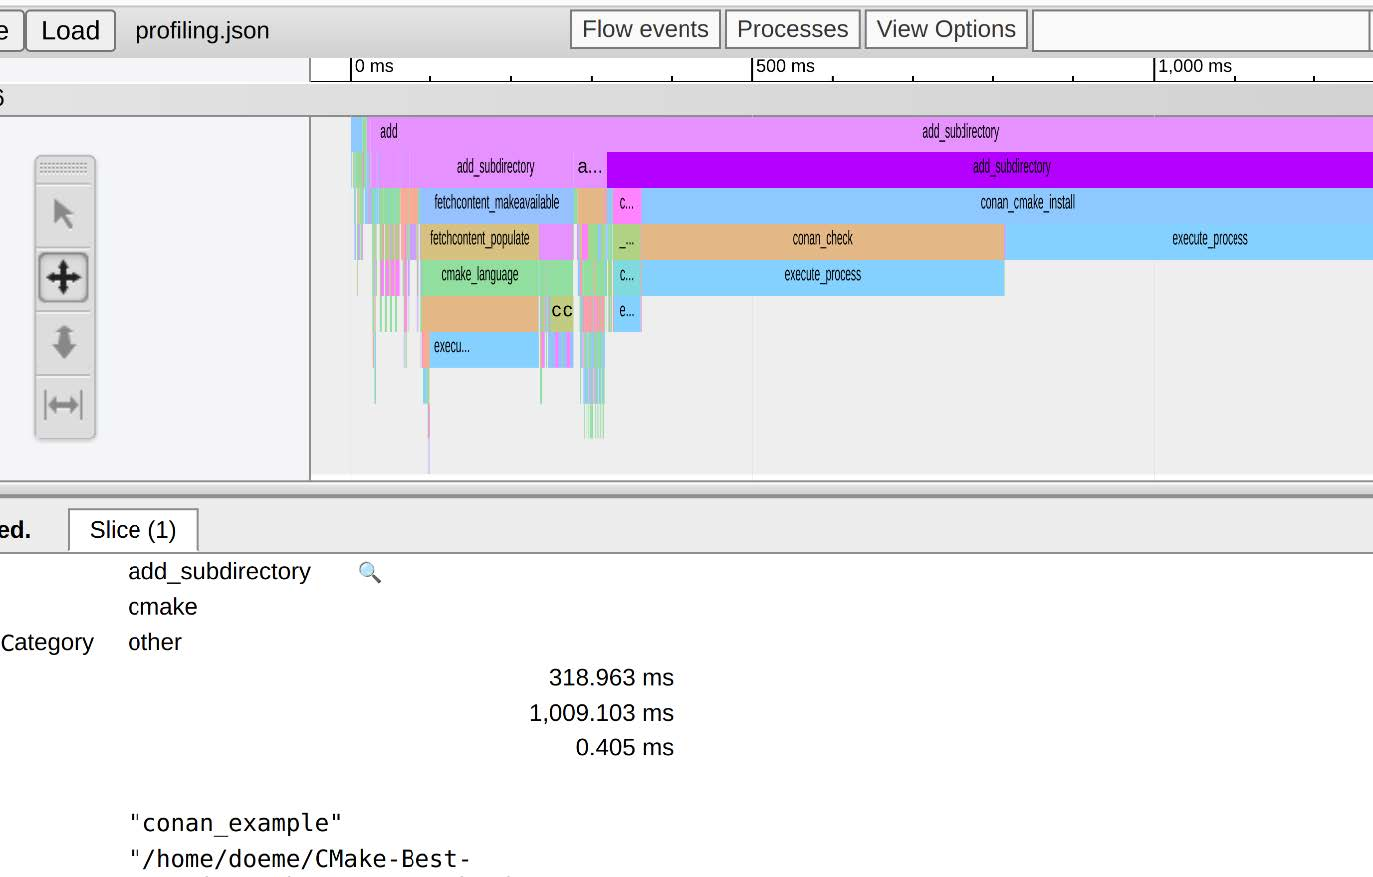
\includegraphics[width=0.8\textwidth]{content/3/chapter14/images/1.jpg}\\
图14.1  CMake项目在Google Chrome中的概要图示例
\end{center}

配置项目时,有个\texttt{add\_subdirectory}占用了大部分时间。本例中,这是chapter05子目录,需要3秒多一点的时间来完成。深入研究一下,就会发现这些例子都使用了Conan包管理器,即两次调用conan\_cmake\_install使得配置的开销相对较大,将对Conan的调用集中到一个更高的目录中,可以将CMake的配置运行时间减少一半。

为了正确地解释分析输出,有助于相互比较不同的CMake运行情况,特别是将CMake运行在干净的缓存上与使用缓存信息的缓存上进行比较。若CMake只在干净的缓存上运行,但增量运行足够快,这对开发人员来说仍然可以接受。然而,若增量CMake运行也需要很久,这可能会造成更大的问题。分析它们可以确定每次运行配置时是否执行了不必要的步骤。

修复缓慢的构建步骤取决于具体的情况,但配置时间过长的常见原因是每次都要下载文件,因为一开始没有检查文件是否存在。分析可能经常会发现,像\texttt{execute\_process}或\texttt{try\_compile}这样的指令占用了大量的执行时间。最简单的“解决方法”是尝试摆脱这些调用,但这些调用的存在往往是有原因的。通常情况下,跟踪指令的堆栈会找到降低调用这些函数频率的方法。结果进行缓存,或者用\texttt{execute\_process}创建的文件不需要每次都生成。

特别是在交叉编译时,\texttt{find\_}指令可能也会占用大量时间。如第5章所述,通过改变CMAKE\_FIND\_ROOT\_PATH\_MODE\_*变量来改变搜索顺序,可能会有所帮助。要更彻底地分析为什么\texttt{find\_}会占用太多时间,可以通过将CMAKE\_FIND\_DEBUG\_MODE变量设置为true,来告诉CMake启用相应的调试输出。由于这将打印出很多信息,因此最好只对某些调用启用此选项,如下所示:

\begin{lstlisting}[style=styleCMake]
set(CMAKE_FIND_DEBUG_MODE TRUE)
find_package(...)
set(CMAKE_FIND_DEBUG_MODE FALSE)
\end{lstlisting}

CMake的配置选项允许对构建过程的配置阶段进行配置,必须使用相应的生成器来分析实际的编译和时间。大多数生成器要么支持一些分析选项,要么记录所需的信息。对于Visual Studio生成器,vcperf工具(\url{https://github.com/microsoft/vcperf})将提供很多信息。使用Ninja时,可以使用ninjatracing工具(\url{https://github.com/nico/ninjatracing})将.ninja\_log文件转换为Google跟踪格式。虽然CMake不支持分析软件的实际编译和链接,但它提供了改进构建时间的方法,我们将在下一节中看到。































